\documentclass[a4paper, 11pt]{article}
\usepackage{comment} % enables the use of multi-line comments (\ifx \fi) 
\usepackage{xparse}% http://ctan.org/pkg/xparse
\NewDocumentCommand{\Log}{o}{%
  \IfNoValueTF{#1}{}{{}^{#1}\!}\log}%
  
\usepackage{fullpage} % changes the margin
\usepackage{longtable}
\usepackage{graphicx}
\usepackage{fancyvrb,xcolor}
\usepackage{listings}
\usepackage{color}
\usepackage[hyphenbreaks]{breakurl}
\usepackage[hyphens]{url}
\usepackage[margin=3cm]{geometry}
\usepackage{relsize}
\definecolor{dkgreen}{rgb}{0,0.6,0}
\definecolor{gray}{rgb}{0.5,0.5,0.5}
\definecolor{mauve}{rgb}{0.58,0,0.82}
\usepackage{float}
\usepackage{caption}
\DeclareCaptionFont{white}{\color{white}}
\DeclareCaptionFormat{listing}{\colorbox{gray}{\parbox{\textwidth}{#1#2#3}}}
\captionsetup[lstlisting]{format=listing,labelfont=white,textfont=white}
\newcommand{\bigqm}[1][1]{\text{\larger[#1]{\textbf{?}}}}
\lstset{
  language=Java,
  aboveskip=3mm,
  belowskip=3mm,
  showstringspaces=false,
  columns=flexible,
  basicstyle={\small\ttfamily},
  numbers=none,
  numberstyle=\tiny\color{gray},
  keywordstyle=\color{blue},
  commentstyle=\color{dkgreen},
  stringstyle=\color{mauve},
  breaklines=true,
  breakatwhitespace=true,
  tabsize=3
}
\graphicspath{ {images/} }

\begin{document}
%Header-Make sure you update this information!!!!
\noindent
\large\textbf{Assignment 10} \hfill \textbf{Hussam Hallak} \\
\normalsize CS532, Web Science, Spring 2017\hfill CS Master's Student \\
Old Dominion University, Computer Science Dept \hfill Prof: Dr. Nelson 

\section*{Question 1:}
Using the data from A8:

- Consider each row in the blog-term matrix as a 1000 dimension vector, 
corresponding to a blog.  

- From chapter 8, replace numpredict.euclidean() with cosine as the 
distance metric.  In other words, you'll be computing the cosine between
vectors of 1000 dimensions.  

- Use knnestimate() to compute the nearest neighbors for both:

http://f-measure.blogspot.com/
http://ws-dl.blogspot.com/

for k={1,2,5,10,20}.


\subsection*{Answer:}

In order to compute the nearest neighbors to both blogs, F-Measure and WSDL, using knnestimate() using the cosine between the vectors to compute the distance instead of the euclidean function, I created a python script, ``knn.py''. The script takes a blog term matrix as command line argument for its input, saved in a file ``blogdata.txt'' copied from Assignment 8. The functions used in the script were taken from ``PCI'' book with small modifications. I utilized ``Scipy'' module to calculate the cosine distance. I saved the output to a file and named it ``knn.txt''.

\lstinputlisting[language=Python, breakatwhitespace=〈false), label=The content of knn.py, caption= The content of knn.py]{Q1/knn.py}

\begin{lstlisting}[language=bash, breakatwhitespace=〈false), label=Running knn.py, caption= Running knn.py]
root@ima-app:/var/www/Hussam/A10# python knn.py blogdata.txt > knn.txt
\end{lstlisting}

\lstinputlisting[language=bash, breakatwhitespace=〈false), label=The Output (the content of knn.txt), caption= The Output (the content of knn.txt)]{Q1/knn.txt}

\subsection*{Included Files:}
knn.py, blogdata.txt, knn.txt

\section*{Question 2:}

Rerun A9, Q2 but this time using LIBSVM.  If you have n categories,
you'll have to run it n times.  For example, if you're classifying music
and have the categories:

metal, electronic, ambient, folk, hip-hop, pop

you'll have to classify things as:

metal / not-metal
electronic / not-electronic
ambient / not-ambient

etc.

Use the 1000 term vectors describing each blog as the features, and
your mannally assigned classifications as the true values.  Use
10-fold cross-validation (as per slide 46, which shows 4-fold
cross-validation) and report the percentage correct for 
each of your categories.

\subsection*{Answer:}

I spent so much time trying to install LIBSVM in so many different ways on multiple computers with different operating systems, but was not successful. This part of the assignment is rather simple, but the technical difficulties are making it hard. I moved on to the next question. 


\section*{Question 3:}

Re-download the 1000 TimeMaps from A2, Q2.  Create a graph where
the x-axis represents the 1000 TimeMaps.  If a TimeMap has "shrunk",
it will have a negative value below the x-axis corresponding to the
size difference between the two TimeMaps.  If it has stayed the
same, it will have a "0" value.  If it has grown, the value will be 
positive and correspond to the increase in size between the two
TimeMaps.

As always, upload all the TimeMap data.  If the A2 github has the 
original TimeMaps, then you can just point to where they are in 
the report.

\subsection*{Answer:}

Similar to my solution for Assignment 2. In fact, copying from there, I performed the following steps:

1. Downloading the TimeMaps for each of the target URIs using the ODU 
Memento Aggregator. I used the same python script from Assignment 2 to do that ``downloadtimemapsjson.py''. The script takes three command line arguments, an input file that has the links for which we want to download the TimeMaps ``uniquelinks.txt'', an output file to store the downloaded TimeMaps, ``timemap.jsonx'' where ``x'' is a number that identifies the timemap (e.g., 1, 2, 3, ...), and another output file, ``uniquelinkswithmemes.txt'', to store the unique links with mementos in.

\textbf{Note:} The number of output files named , ``timemap.jsonx'' may not be the same as the number of links in the input file ``uniquelinks.txt''. The reason is because not all links have mementos.

\lstinputlisting[language=python, label=downloadtimemapsjson.py, caption=The content of downloadtimemapsjson.py, breakatwhitespace=〈false)]{Q3/downloadtimemapsjson.py}

\begin{lstlisting}[language=bash, breakatwhitespace=〈false), label=Command, caption=Running downloadtimemapsjson.py]
root@ima-app:/var/www/Hussam/A10# python downloadtimemapsjson.py uniquelinks.txt timemap.json uniquelinkswithmemes.txt
\end{lstlisting}

Now I have 463 links with mementos out of the original 1107 unique links in the input file.

\begin{lstlisting}[language=bash, breakatwhitespace=〈false), label=Command, caption=Links with mementos:]
root@ima-app:/var/www/Hussam/A10# cat uniquelinks.txt | wc -l
1107
root@ima-app:/var/www/Hussam/A10# cat uniquelinkswithmemes.txt | wc -l
463
root@ima-app:/var/www/Hussam/A10# ls timemap.json* | wc -l
463
\end{lstlisting}

2. Parse the downloaded TimeMaps, JSON files, to find the number of mementos for each URI that has a TimeMap. I used the same Python script I wrote for Assignment 2, ``parsejsontimemap.py'', with some modification to do that. The script loops over all TimeMaps' files ``timemap.jsonx'' and parses them to find the number of mementos for each link and saves the link with its number of mementos in an output file named ``linksnmemesnumA10.txt''. The program also saves the number of mementos only in a file as output, ``timemapreport.txt''. This is the file that I will use to generate a histogram in R in the next step. The file ``linksnmemesnumA10.txt'' will later be used to generate the desired graph in this assignment that compares the results from this assignment with the results from Assignment 2. I had to run the script ``parsejsontimemap.py'' on the timemaps from Assignment 2 to generate ``linksnmemesnumA2.txt'' as well.

\lstinputlisting[language=python, label=parsejsontimemap.py, caption=The content of parsejsontimemap.py, breakatwhitespace=〈false)]{Q3/parsejsontimemap.py}

\begin{lstlisting}[language=bash, breakatwhitespace=〈false), label=Command, caption=Running parsejsontimemap.py]
root@ima-app:/var/www/Hussam/A10# python parsejsontimemap.py timemap.json timemapreport.txt
root@ima-app:/var/www/Hussam/A10# cat timemapreport.txt | wc -l
463
\end{lstlisting}

3. Now we are ready to generate the histogram for URIs vs. the number of Mementos in R.

This line of code reads the data in the file and stores it in the vector timemaps\_data.
\begin{lstlisting}
> timemaps_data <- read.table("C:/R/timemapreport.txt", header=F, sep="\t")
\end{lstlisting}

This line of code defines a variable max\_num and assigns the maximum value in the vector timemaps\_data to it.
\begin{lstlisting}
> max_num <- max(timemaps_data)
\end{lstlisting}

This line of code creates a histogram for timemaps\_data  with fire colors, sets bin = 1 so each number is in its own group, makes x axis range from 0 to max\_num, disables right-closing of cell intervals, sets heading, changes the label of the x-axis, and makes y-axis labels horizontal
\begin{lstlisting}
> hist(timemaps_data[,1], col=heat.colors(max_num), breaks=max_num, xlab="Number of Mementos", xlim=c(0,max_num), right=F, main="Mementos Histogram", las=1)
\end{lstlisting}

\begin{figure}[H]
\centering
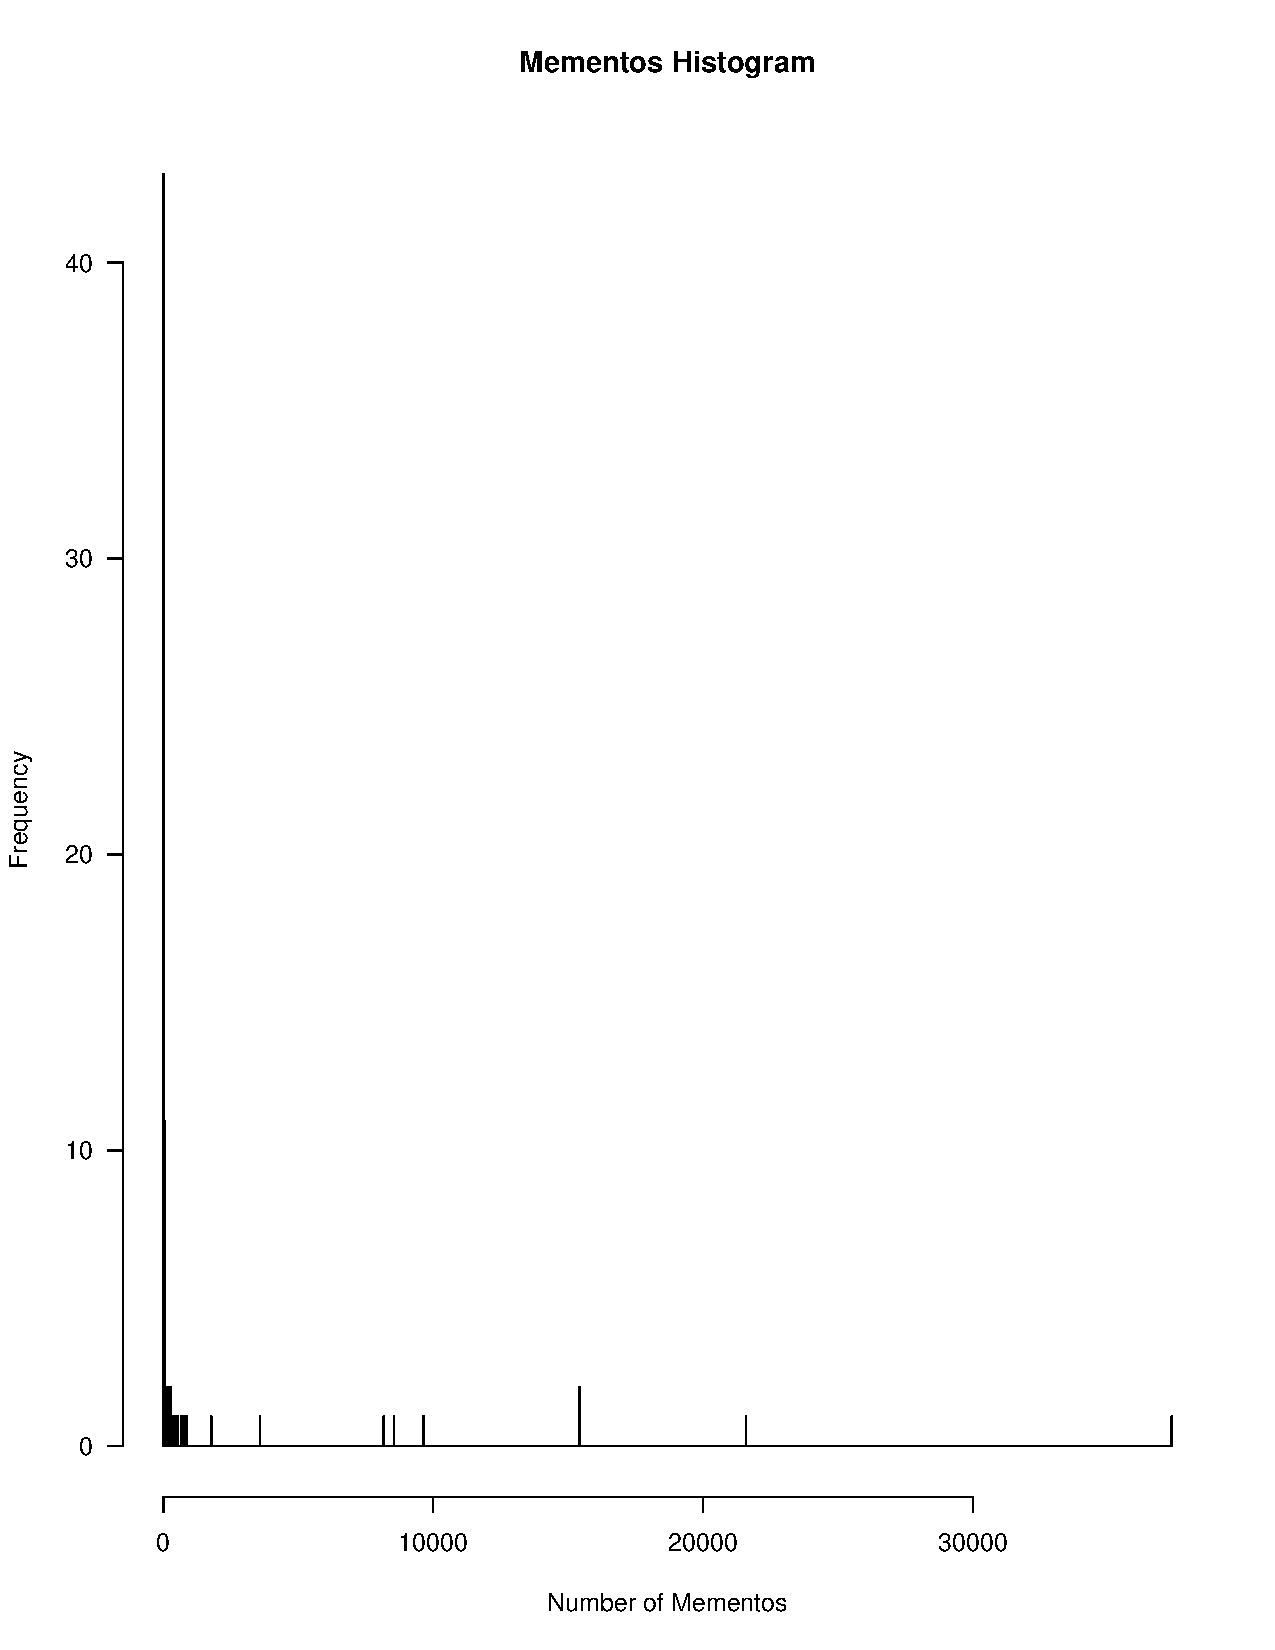
\includegraphics[scale=0.7]{hist1.pdf}
\end{figure}
\pagebreak

We notice that our histogram did not provide a good representation of the results. I am going to zoom into the part where most of the data is and exclude the outliars in the data. Modifying the last line of code to this one will do just that.

\begin{lstlisting}
>  hist(timemaps_data[,1], col=heat.colors(max_num/500), breaks=max_num, xlab="Number of Mementos", xlim=c(0,max_num/500), right=F, main="Mementos Histogram", las=1)
\end{lstlisting}

\begin{figure}[H]
\centering
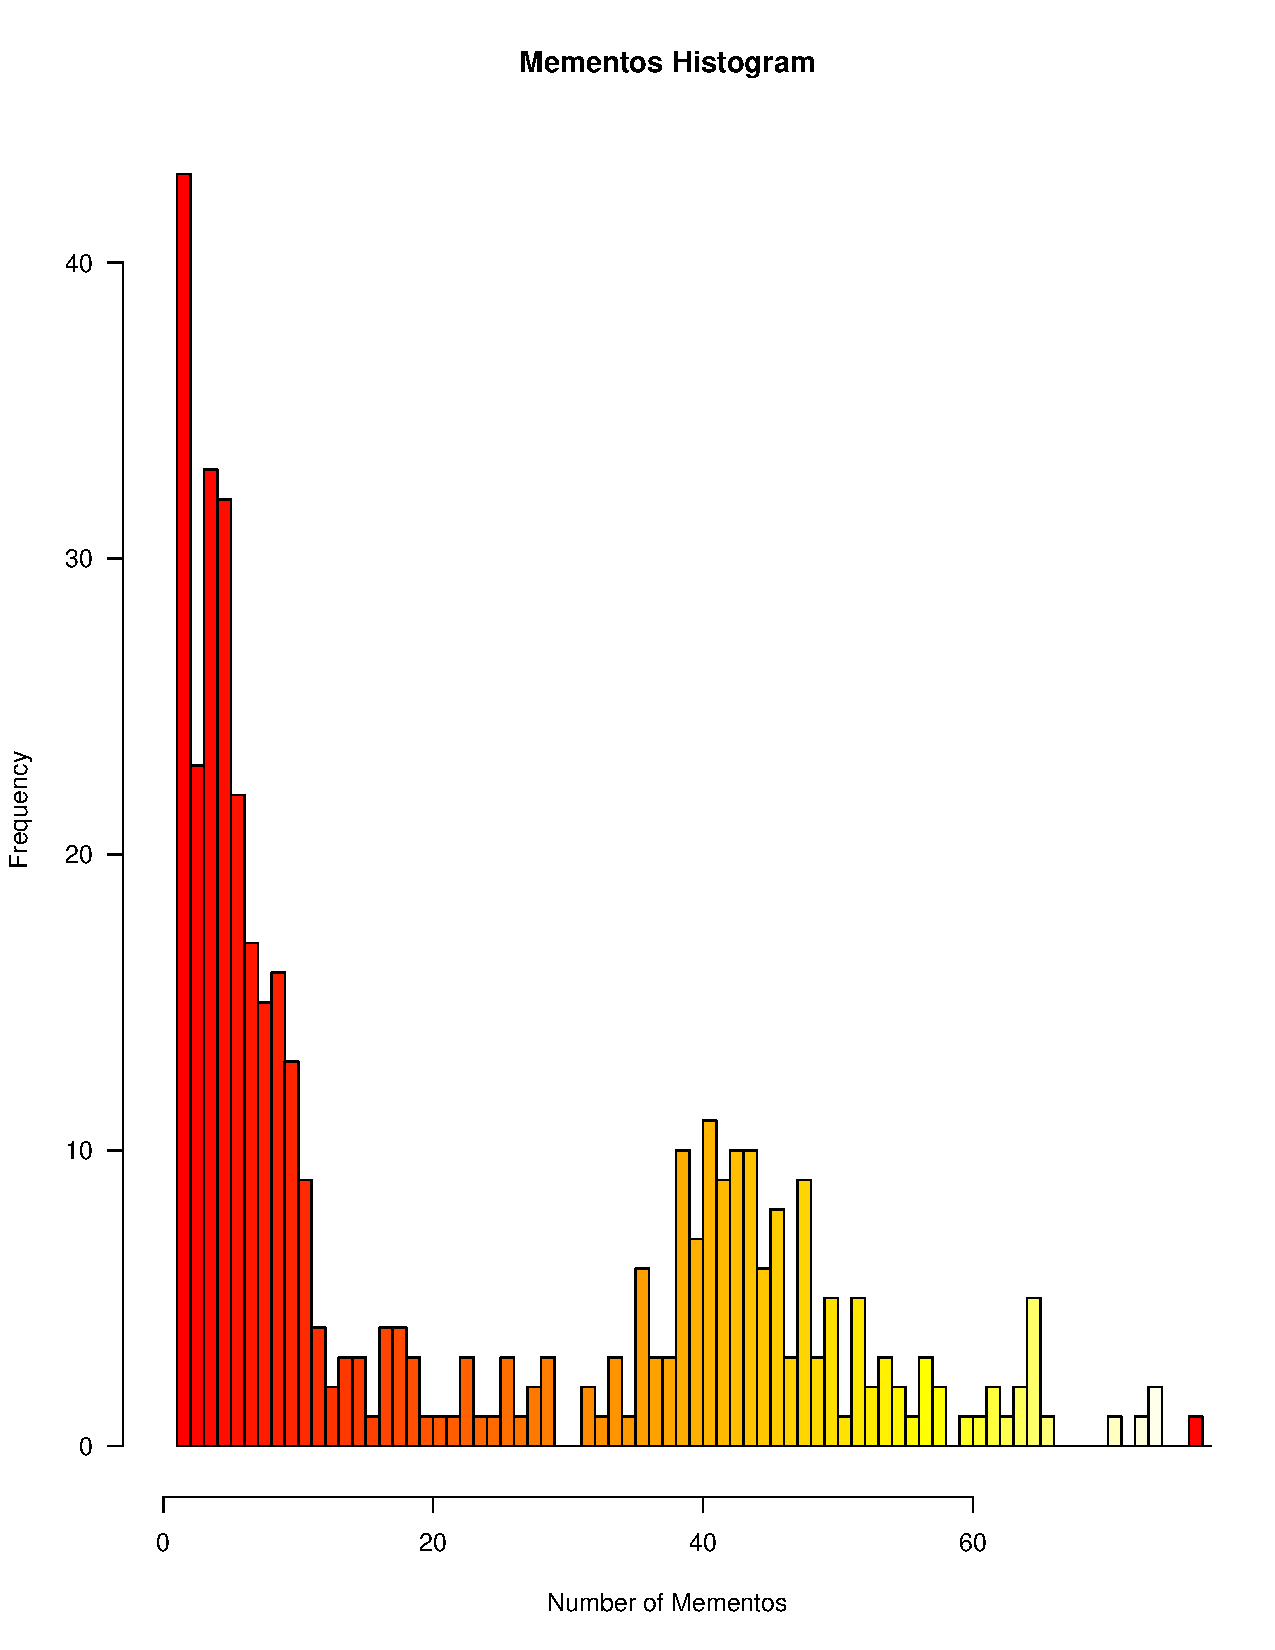
\includegraphics[scale=0.7]{hist2.pdf}
\end{figure}
\pagebreak

4. In order to create a graph where the x-axis represents the 1000 TimeMaps comparing the results from Assignment 2 to this assignment, I wrote a python script, ``comparetm.py'', to do that. The script takes two command line arguments, which contain the data, in this case ``linksnmemesnumA2.txt'' and ``linksnmemesnumA10.txt''. It subtracts the number of mementos for each URI and saves the results to an output file named ``graphtm.txt''. This file will be used to generate the desired graph in this question.

\lstinputlisting[language=python, label=parsejsontimemap.py, caption=The content of comparetm.py, breakatwhitespace=〈false)]{Q3/comparetm.py}

\begin{lstlisting}[language=bash, breakatwhitespace=〈false), label=Command, caption=Running comparetm.py]
root@ima-app:/var/www/Hussam/A10# python comparetm.py linksnmemesnumA2.txt linksnmemesnumA10.txt
\end{lstlisting}

We are finally ready to create the desired graph in R. This R code does exactly that.

\begin{lstlisting}[language=R, breakatwhitespace=〈false), label=Command, caption=R code to create the graph]
> data <- read.table("C:/R/graphtm.txt")
> plot(data$V1, type="l", main="Timemaps Difference between A2 and A10", col.main="blue", col="green", xlab ="Links",ylab="Timemaps Shrinking/Growing", col.lab="red", ylim=c(-2000,2000))
\end{lstlisting}
Here is the desired graph that shows the difference in the number of mementos between Assignment 2 and this assignment.

\begin{figure}[H]
\centering
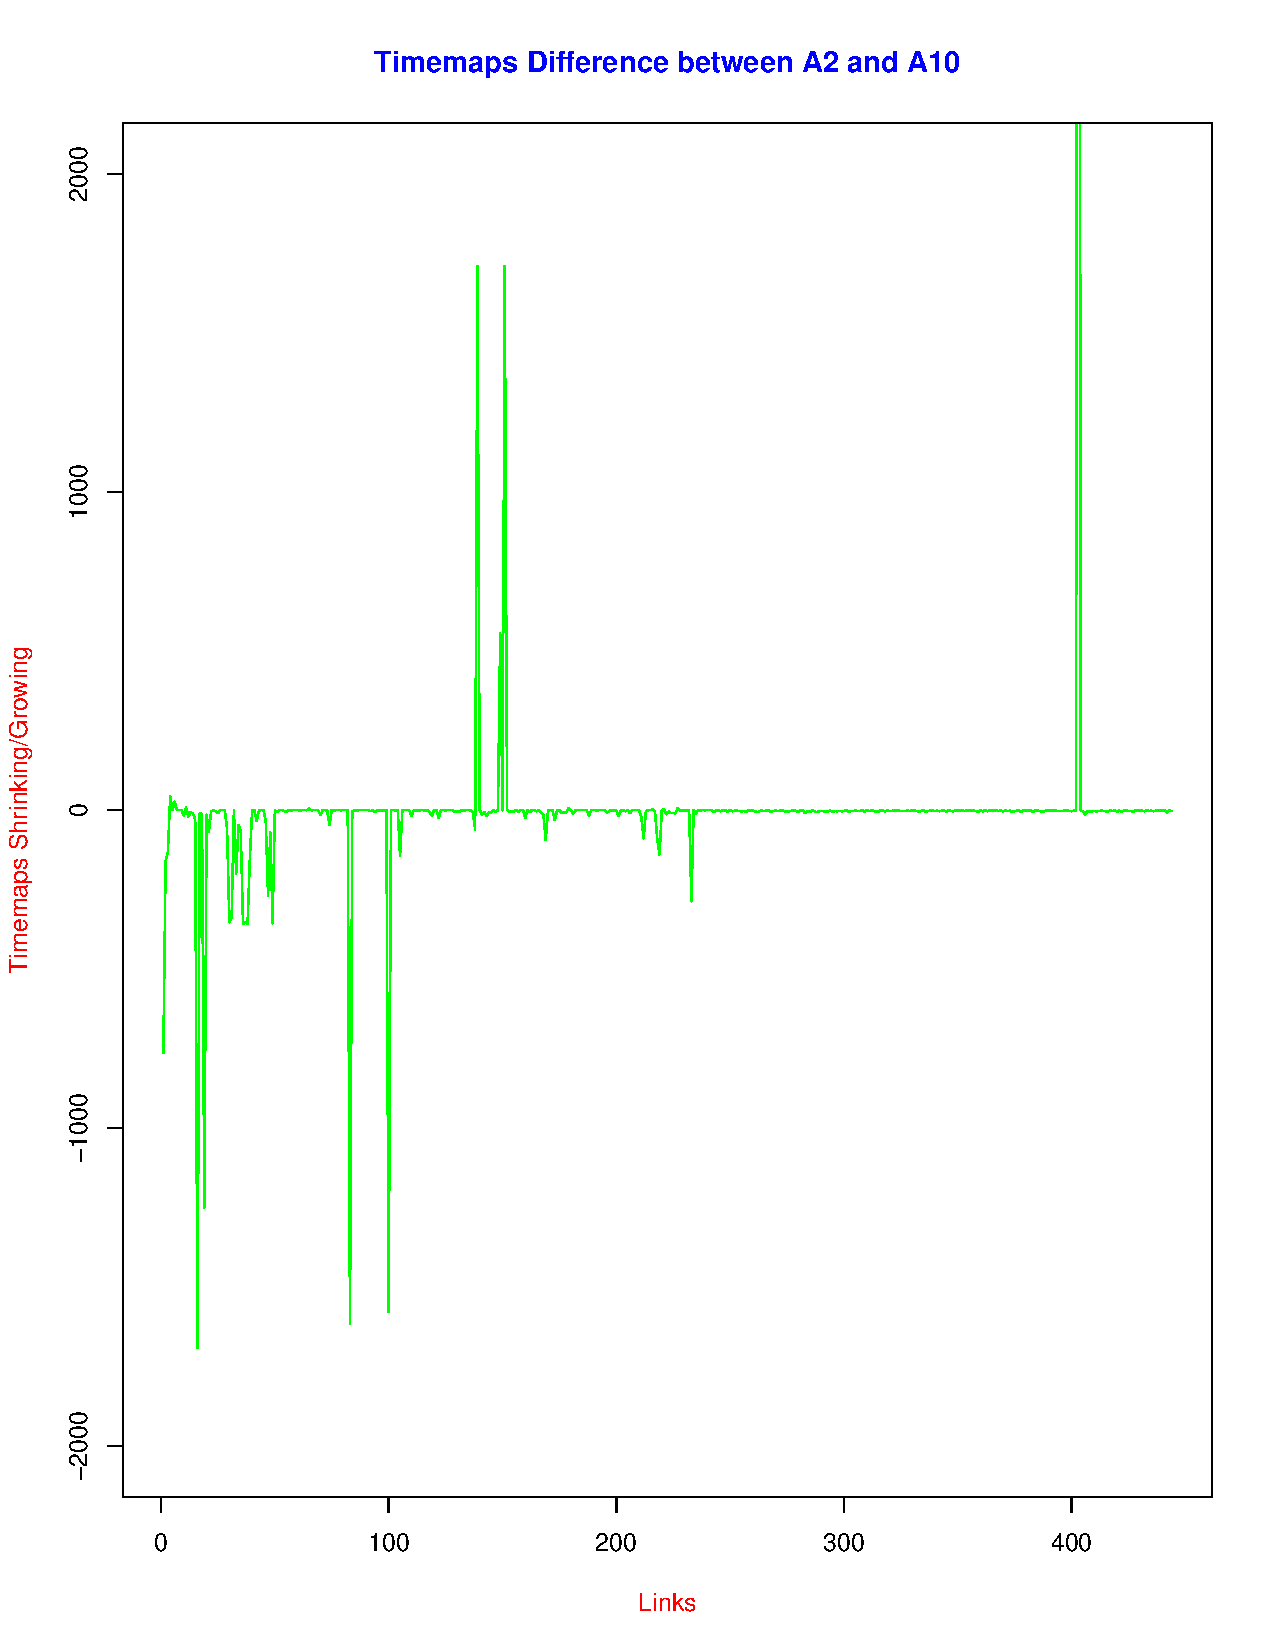
\includegraphics[scale=0.5]{graphtm.pdf}
\end{figure}

\subsection*{Included Files:}
downloadtimemapsjson.py, uniquelinks.txt, uniquelinkswithmemes.txt, parsejsontimemap.py, timemapreport.txt, linksnmemesnumA10.txt, linksnmemesnumA2.txt, comparetm.py, graphtm.txt, hist1.pdf, hist2.pdf, graphtm.pdf 

\noindent 
Folder: timemaps that has all timemap.json* files, 


\section*{Question 4:}

Repeat A3, Q1.  Compare the resulting text from February to 
the text you have now.  Do all 1000 URIs still return a "200 OK" 
as their final response (i.e., at the end of possible redirects)?

Create two graphs similar to that described in Q3, except this 
time the y-axis corresponds to difference in bytes (and not difference
in TimeMap magnitudes).  For the first graph, use the difference
in the raw (unprocessed) results.  For the second graph, use the 
difference in the processed (as per A3, Q1) results.

Of the URIs that still terminate in a "200 OK" response, pick the
top 3 most changed (processed) pairs of pages and use the Unix
"diff" command to explore the differences in the version pairs.

\subsection*{Answer:}

Similar to what I did in Assignment 3, the approach is divided into two steps:

1. Take the unique links collected from Assignment 2, saved in ``uniquelinks.txt'' and download their content, then save it to text files, one file for each link. For that purpose I used md5 hashing to name the output files.

2. Remove (most) of the HTML markup from the content of the downloaded HTML pages.

I wrote a python script, ``parselinks.py'', that will combine both steps. First it will download the raw HTML for each link and save it to a file, then it will strip HTML markup and save it to another file with the same name postfixed with ``.processed''. The program will also create a text file named ``map.txt'' to map each link to its new file name.

\lstinputlisting[language=Python, breakatwhitespace=〈false), label=parselinks.py, caption=The content of parselinks.py]{Q4/parselinks.py}

\begin{lstlisting}[language=bash, breakatwhitespace=〈false), label=running parselinks.py, caption= Running parselinks.py to download raw HTML and visible text from URIs]
root@ima-app:/var/www/Hussam/A10/Q4# python parselinks.py uniquelinks.txt
root@ima-app:/var/www/Hussam/A10/Q4# ls | wc -w
799
\end{lstlisting}


The program created 796 output files, two files for each link. This means that the content of 398 URIs was downloaded and processed successfully. The rest of the links generated errors. That could be due to different reasons including bad HTML markup, the page no longer exists on the web, or other reasons. The interesting part is that the number of URIs that were downloaded and processed successfully at the time I did Assignment 3 was 397 which is one URI less than this time, Assignment 10. The only explanation I can think of is that one or more URIs were not available at the time I did Assignment 3 and now they are, or bad HTML in one of the URIs that has been fixed since I did Assignment 3. Most of the links I collected belong to famous news channels which explains why most, if not all, of the ones that returned "200 OK" in Assignment 3 returned "200 OK" now.

The next step is creating the graphs. I wrote a python script, ``comparefiles.py'', that will compare the sizes of files that belong to each URI. The program does that for both the raw and the processed files. The script accepts one command line argument, that is ``map.txt'' in our case to get the file names, then it finds the sizes for both old and new files in both cases raw and processed. The program then subtracts the sizes and saves the difference between the raw files to ``rawdiff.txt'' and the difference between the processed files to ``processeddiff.txt''. These two files will be used to generate our graphs in R. 

I copied the raw and processed files from Assignment 3 to the folders ``rawold'' and ``processedold'' respectively. I also copied the newly created raw and processed files, from this assignment, to the folders ``rawnew'' and ``processednew'' respectively. This will make things more organized for the script ``comparefiles.py''. 

\lstinputlisting[language=Python, breakatwhitespace=〈false), label=comparefiles.py, caption=The content of comparefiles.py]{Q4/comparefiles.py}

\begin{lstlisting}[language=bash, breakatwhitespace=〈false), label=running comparefiles.py, caption= Running comparefiles.py to create the files rawdiff.txt and processeddiff.txt to generate the graphs in R.]
root@ima-app:/var/www/Hussam/A10/Q4# python comparefiles map.txt
\end{lstlisting}

We are now ready to create the desired graph for raw files in R. This R code does exactly that.

\begin{lstlisting}[language=R, breakatwhitespace=〈false), label=Command, caption=R code to create the graph]
> data <- read.table("C:/R/rawdiff.txt")
> plot(data$V1, type="l", main="Size Difference in Bytes for Raw Files between A2 and A10", col.main="blue", col="green", xlab ="Links",ylab="Size Difference in Bytes", col.lab="red", ylim=c(-20000,20000))
\end{lstlisting}
   
\begin{figure}[H]
\centering
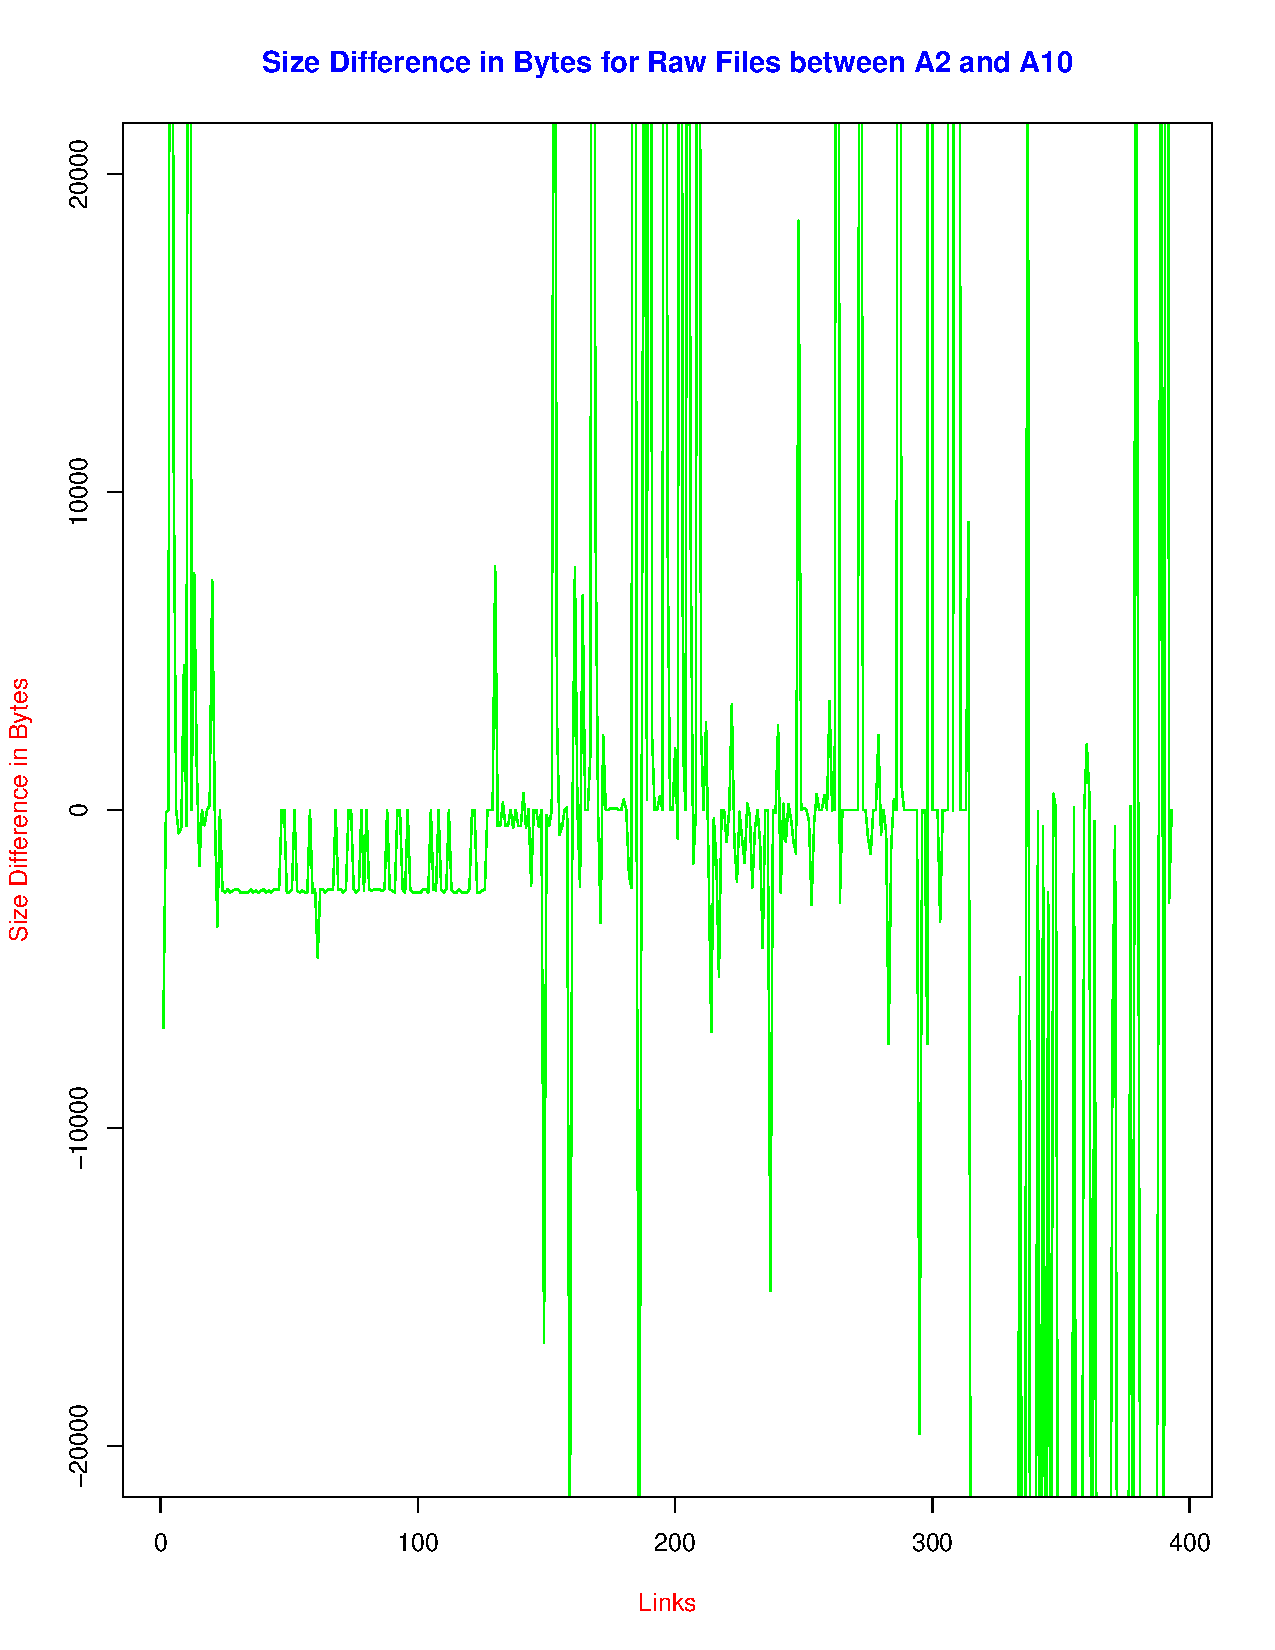
\includegraphics[scale=0.5]{rawdiff.pdf}
\end{figure}

In a similar fashion, I created the desired graph for processed files in R.

\begin{lstlisting}[language=R, breakatwhitespace=〈false), label=Command, caption=R code to create the graph]
> data <- read.table("C:/R/processeddiff.txt")
> plot(data$V1, type="l", main="Size Difference in Bytes for Processed Files between A2 and A10", col.main="blue", col="green", xlab ="Links",ylab="Size Difference in Bytes", col.lab="red", ylim=c(-2000,2000))
\end{lstlisting}
   
\begin{figure}[H]
\centering
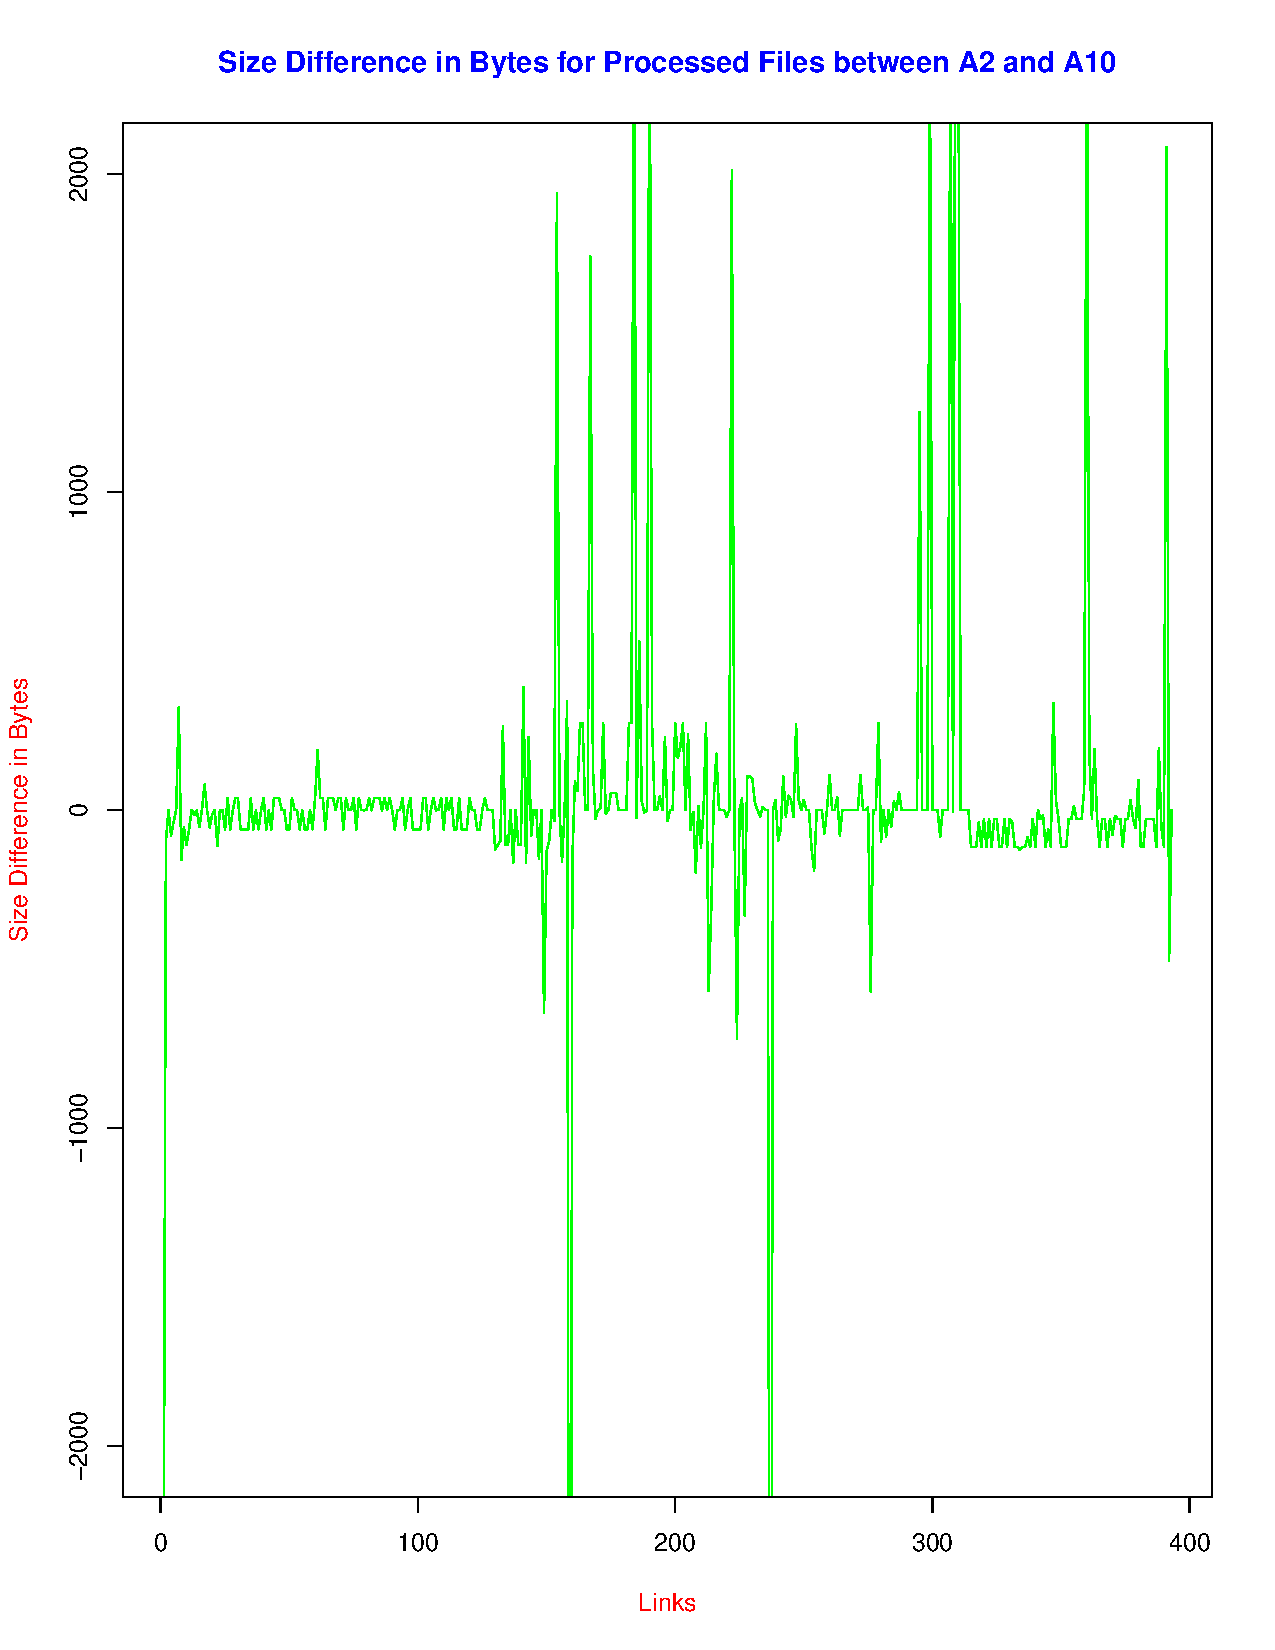
\includegraphics[scale=0.5]{processeddiff.pdf}
\end{figure}


Now let's pick the top 3 most changed (processed) pairs of pages per the requirements in the question. I created a small php script, ``top3.php'', to help me do that. The script takes a command line argument as input, it is the file ``map.txt'', which maps each link to the name of its processed file. It extracts all the processed file names and computes the size difference in bytes between each pair of processed files from Assignment 3 and the files created in this assignment. It saves these values in an associative array with the file name as the key, and the difference in bytes as the value. Then it sorts the array by the value maintaining index association, keeping the (key,value) together. Finally, the sorted array that has the file names along with the difference in bytes is sent as an output to a file named ``sizedifference.txt''. 

\lstinputlisting[language=php, breakatwhitespace=〈false), label=top3.php, caption=The content of top3.php]{Q4/top3.php}

\begin{lstlisting}[language=bash, breakatwhitespace=〈false), label=running top3.php, caption= Running top3.php to sort the processed files based on the difference in size]
root@ima-app:/var/www/Hussam/A10/Q4# php top3.php map.txt
\end{lstlisting}

In order to pick top 3 most changed (processed) pairs of pages, I executed the following command to show me the last 3 lines in the file ``sizedifference.txt''.

\begin{lstlisting}[language=bash, breakatwhitespace=〈false), label=Using tail on sizedifference.txt, caption= Using tail on sizedifference.txt to pick top 3 most changed (processed) pairs of pages.]
root@ima-app:/var/www/Hussam/A10/Q4# tail sizedifference.txt -n 3
79c8e70bf1211bc717dca09b66a27aef.processed --> 11558
29c1253c338efaad05365a28c1b25495.processed --> 17381
68046d7c24bb2dacd6dc28333caa0625.processed --> 25594
root@ima-app:/var/www/Hussam/A10/Q4#
\end{lstlisting}


\subsection*{Included Files:}
parselinks.py, uniquelinks.txt, map.txt, comparefiles.py, rawdiff.txt, processeddiff.txt. top3.php, sizedifference.txt, rawdiff.pdf, processeddiff.pdf

\noindent
Folder ``rawold'' contains all raw HTML files from Assignment 3
 
\noindent
Folder ``processedold'' contains all visible text in HTML files from Assignment 3

\noindent
Folder ``rawnew'' contains all raw HTML files from this assignment
 
\noindent
Folder ``processednew'' contains all visible text in HTML files from this assignment

\end{document}
